\whiteBGstarBegin
\setcounter{section}{0}
\section{Trắc nghiệm}
\begin{enumerate}[label=\bfseries Câu \arabic*:]
	

\item \mkstar{1}

\cauhoi
{Chuyển động của vật nào dưới đây được coi là chuyển động tròn đều?
	\begin{mcq}
		\item Chuyển động của bánh xe ô tô khi đang hãm phanh.
		\item Chuyển động của kim phút trên mặt đồng hồ chạy đúng giờ.
		\item Chuyển động quay của các điểm treo các ghế ngồi trên chiếc đu quay.
		\item Chuyển động quay của cánh quạt khi vừa tắt điện.
	\end{mcq}
	
}
\loigiai
{	\textbf{Đáp án: B.}
	
	Chuyển động của kim phút trên mặt đồng hồ chạy đúng giờ là chuyển động tròn đều.
}
\item \mkstar{1}

\cauhoi
{Các công thức liên hệ giữa tốc độ góc $\omega$ với chu kỳ $T$ và giữa tốc độ góc $\omega$ với tần số $f$ trong chuyển động tròn đều là gì?
	\begin{mcq}(2)
		\item $\omega=2\pi T$; $\omega=\dfrac{2\pi}{f}$.
		\item $\omega=\dfrac{2\pi}{T}$; $\omega=2\pi f$.
		\item $\omega=2\pi T$; $\omega=2\pi f$. 
		\item $\omega=\dfrac{2\pi}{T}$; $\omega=\dfrac{2\pi}{f}$.
	\end{mcq}
	
}
\loigiai
{	\textbf{Đáp án: B.}
	
	Công thức liên hệ giữa tốc độ góc $\omega$ với chu kỳ $T$ là $\omega=\dfrac{2\pi}{T}$.
	Công thức liên hệ giữa giữa tốc độ góc $\omega$ với tần số $f$ trong chuyển động tròn đều là $\omega=2\pi f$.
}


\item \mkstar{2}

\cauhoi
{Một bánh xe có đường kính $\SI{100}{\centi\meter}$ lăn đều với vận tốc $\SI{36}{\kilo\meter/\hour}$. Gia tốc hướng tâm của một điểm trên vành bánh xe có độ lớn
	\begin{mcq}(4)
		\item $\SI{200}{\meter/\second^2}$.
		\item $\SI{400}{\meter/\second^2}$.
		\item $\SI{100}{\meter/\second^2}$.
		\item $\SI{300}{\meter/\second^2}$.
	\end{mcq}
}
\loigiai
{	\textbf{Đáp án: A.}
	
	Đổi đơn vị: $\SI{100}{\centi\meter}=\SI{1}{\meter}$; $\SI{36}{\kilo\meter/\hour}=\SI{10}{\meter/\second}$
	
	Gia tốc hướng tâm của một điểm trên vành bánh xe có độ lớn:
	$$a_\text{ht}=\dfrac{v^2}{R}=\SI{200}{\meter/\second^2}.$$
}

\item \mkstar{2}

\cauhoi
{Một đĩa tròn bán kính $\SI{20}{\centi\meter}$ quay đều quanh trục của nó. Đĩa quay hết 1 vòng mất $\SI{0.2}{\second}$. Tốc độ dài $v$ của một điểm nằm ở mép đĩa bằng
	\begin{mcq}(4)
		\item $\SI{4,71}{\meter/\second}$. 
		\item $\SI{3,14}{\meter/\second}$. 
		\item $\SI{6,28}{\meter/\second}$. 
		\item $\SI{7,85}{\meter/\second}$.
	\end{mcq}
	
}
\loigiai
{	\textbf{Đáp án: C.}
	
	Tốc độ dài $v$ của một điểm trên vành ngoài xe:
	$v=r\omega=r\dfrac{\Delta \alpha}{\Delta t}=\SI{0,2}{\meter}\dfrac{2\pi}{\SI{0.2}{\second}}=\SI{6,28}{\meter/\second}$
}
\item \mkstar{2}

\cauhoi
{Một động cơ xe máy có trục quay 1200 vòng/phút. Tốc độ góc của chuyển động quay là bao nhiêu?
	\begin{mcq}(4)
		\item $\SI{125,7}{\radian/\second}$.
		\item $\SI{188,5}{\radian/\second}$.
		\item $\SI{62,8}{\radian/\second}$.
		\item $\SI{7200}{\radian/\second}$.
	\end{mcq}
}
\loigiai
{	\textbf{Đáp án: A.}
	
	Tốc độ góc của chuyển động quay là:
	$\omega$ = 1200 vòng/ phút = $1200\cdot\dfrac{2\pi}{60}\,\SI{}{\radian/\second}=\SI{125,7}{\radian/\second}$
}
\item \mkstar{2}

\cauhoi
{Một bánh xe có bán kính $\SI{100}{\centi\meter}$ lăn đều với vận tốc $\SI{54}{\kilo\meter/\hour}$. Gia tốc hướng tâm của một điểm trên vành bánh xe có độ lớn
	\begin{mcq}(4)
		\item $\SI{225}{\meter/\second^2}$.
		\item $\SI{400}{\meter/\second^2}$.
		\item $\SI{100}{\meter/\second^2}$.
		\item $\SI{300}{\meter/\second^2}$.
	\end{mcq}
}
\loigiai
{	\textbf{Đáp án: A.}
	
	Gia tốc hướng tâm của một điểm trên vành bánh xe có độ lớn:
	$$a_\text{ht}=\dfrac{v^2}{R}=\SI{225}{\meter/\second^2}.$$
}

\item \mkstar{3}

\cauhoi
{Một vệ tinh nhân tạo ở độ cao $\SI{250}{\kilo\meter}$ bay quanh Trái Đất theo một quỹ đạo tròn. Chu kì của vệ tinh là 88 phút. Tính gia tốc hướng tâm của vệ tinh. Cho bán kính Trái Đất là $\SI{6400}{\kilo\meter}$.
	\begin{mcq}(4)
		\item $\SI{9,41}{ \meter/\second^2}$.
		\item $\SI{9,48}{ \meter/\second^2}$.
		\item $\SI{8,72}{ \meter/\second^2}$.
		\item $\SI{10,05}{ \meter/\second^2}$.
	\end{mcq}
}
\loigiai
{	\textbf{Đáp án: A.}
	
	Khoảng cách từ vệ tinh đến tâm Trái Đất: 
	$$r=\SI{250}{\kilo\meter}+\SI{6400}{\kilo\meter} =\SI{6650}{\kilo\meter}=\SI{6650000}{\meter}.$$
	
	Tốc độ góc của vệ tinh:
	$$T=\frac{2\pi}{\omega} \Rightarrow \omega = \frac{\pi}{2640}\ \text{rad/s}.$$ 
	
	Gia tốc hướng tâm của vệ tinh: 
	
	$$a_{ht}=\omega^2 \cdot r \approx \SI{9,41}{ \meter/\second^2}.$$
}
\item \mkstar{3}

\cauhoi
{Xe đạp của một vận động viên chuyển động thẳng đều với $v=\SI{36}{km/h}$. Biết bán kính của lốp xe đạp là $\SI{32.5}{cm}$. Tính tốc độ góc và gia tốc hướng tâm tại một điểm trên lốp bánh xe.
	\begin{mcq}(2)
		\item $\omega = \SI{30.77}{rad/s}$, $a_\text{ht} = \SI{307.7}{m/s^2}$.
		\item $\omega = \SI{30.77}{rad/s}$, $a_\text{ht} = \SI{377.7}{m/s^2}$.
		\item $\omega = \SI{3.77}{rad/s}$, $a_\text{ht} = \SI{30.7}{m/s^2}$.
		\item $\omega = \SI{3.77}{rad/s}$, $a_\text{ht} = \SI{307.7}{m/s^2}$.
	\end{mcq}
}
\loigiai
{	\textbf{Đáp án: A.}
	
	Vận tốc xe đạp cũng là tốc độ dài của một điểm trên lốp xe:
	$$v=\SI{36}{km/h} = \SI{10}{m/s}$$
	
	Tốc độ góc:
	$$\omega = \dfrac{v}{R} = \SI{30.77}{rad/s}$$
	
	Gia tốc hướng tâm:
	$$a_\text{ht} = \dfrac{v^2}{R} = \SI{307.7}{m/s^2}$$
}
\item \mkstar{3}

\cauhoi
{Hai vật A và B chuyển động tròn đều với cùng chu kì trên hai đường tròn có bán kính khác nhau lần lượt là $R_\text A$ và $R_\text B$, với $R_\text A = 4 R_\text B$. Nếu vật A chuyển động với tốc độ dài $\SI{12}{m/s}$ thì tốc độ dài của vật B là
	\begin{mcq}(4)
		\item $\SI{48}{m/s}$.
		\item $\SI{24}{m/s}$.
		\item $\SI{3}{m/s}$.
		\item $\SI{4}{m/s}$.
	\end{mcq}
}
\loigiai
{	\textbf{Đáp án: C.}
	
	Lập tỉ lệ:
	$$\dfrac{v_\text A}{v_\text B} = \dfrac{R_\text B}{R_\text A} = \dfrac{1}{4} \Rightarrow v_\text B =\SI{3}{m/s} $$
}
\item \mkstar{4}

\cauhoi
{Hai vật A và B chuyển động tròn đều trên hai đường tròn tiếp xúc nhau. Chu kì của A là 4 s, còn chu kì của B là 2 s. Biết rằng tại thời điểm ban đầu chúng xuất phát cùng một lúc từ điểm tiếp xúc của hai đường tròn và chuyển động ngược chiều nhau. Khoảng thời gian ngắn nhất để hai vật gặp nhau lần nữa là
	\begin{mcq}(4)
		\item $1\ \text s$.
		\item $2\ \text s$.
		\item $6\ \text s$.
		\item $4\ \text s$.
	\end{mcq}
}
\loigiai
{	\textbf{Đáp án: D.}
	
	Khoảng thời gian ngắn nhất để hai vật gặp nhau lần nữa:
	$$\Delta t = \dfrac{\Delta \varphi_\text A }{\omega_\text A} = \dfrac{\Delta \varphi_\text B }{\omega_\text B}$$
	
	Trong đó $\Delta \varphi_\text A = n \Delta \varphi_\text B$, với $n=2k$ với ($k\in Z$)
	
	Vậy khoảng thời gian ngắn nhất khi $n=2$, khi đó $$\Delta t= 4\ \text s$$
}
\end{enumerate}

\whiteBGstarEnd

\loigiai
{
	\begin{center}
		\textbf{BẢNG ĐÁP ÁN}
	\end{center}
	\begin{center}
		\begin{tabular}{|m{2.8em}|m{2.8em}|m{2.8em}|m{2.8em}|m{2.8em}|m{2.8em}|m{2.8em}|m{2.8em}|m{2.8em}|m{2.8em}|}
			\hline
			1.B  & 2.B  & 3.A  & 4.C  & 5.A  & 6.A  & 7.A  & 8.A  & 9.C  & 10.D  \\
			\hline
			
		\end{tabular}
	\end{center}
}
\section{Tự luận}
\begin{enumerate}[label=\bfseries Câu \arabic*:]
	\item \mkstar{1}
	
	\cauhoi{
		Chuyển động tròn đều là gì? Nêu những đặc điểm của vec-tơ vận tốc của chuyển động tròn đều.
	}
	
	\loigiai{
		
		Chuyển động tròn đều là chuyển động có quỹ đạo tròn và có tốc độ trung bình trên mọi cung tròn là như nhau.
		
		Vec-tơ vận tốc của chuyển động tròn đều có đặc điểm:
		\begin{itemize}
			\item Điểm đặt: trên vật;
			\item Phương: tiếp tuyến với đường tròn quỹ đạo;
			\item Chiều: cùng chiều chuyển động;
			\item Độ lớn: không đổi, được gọi là tốc độ dài. Kí hiệu $v$. Công thức: $v=\dfrac{\Delta s}{\Delta t}$
		\end{itemize}
	}
	
	\item \mkstar{2}
	
	\cauhoi{Một đầu cánh quạt quay với tần số 400 vòng/phút. Cánh quạt dài $\SI{0.8}{m}$. Tính tốc độ dài và tốc độ góc của một điểm ở đầu cánh quạt.}
	\loigiai{
	Ta có tần số:
	$$f=400\ \text{vòng/phút} = \xsi{\dfrac{20}{3}}{\text{vòng/s}}$$
	
	Tốc độ góc của một điểm ở đầu cánh quạt:
	$$\omega = 2\pi f = \SI{41.97}{rad/s}$$
	
	Tốc độ dài:
	$$v=r \omega = \SI{33.5}{m/s}$$
	}
	\item \mkstar{3}
	
	\cauhoi
	{Một vệ tinh nhân tạo có quỹ đạo là một đường tròn cách mặt đất 400 km, quay quanh Trái Đất một vòng hết 90 phút. Gia tốc hướng tâm của vệ tinh là bao nhiêu? Cho bán kính Trái Đất $R=\SI{6389}{km}$.
	}
	\loigiai
	{Ta có chu kì quay của vệ tinh là
		$$T=5400\ \text s$$
		
		Tốc độ góc:
		$$\omega = \dfrac{2\pi}{T} = \SI{1.16e-3}{rad/s}$$
		
		Gia tốc hướng tâm:
		$$a_\text{ht} = \dfrac{(R+h)^2 \omega^2}{R+h} = \SI{9.13}{m/s^2}$$
	}
	\item \mkstar{4}
	
	\cauhoi
	{Một đồng hồ treo tường có kim phút dài 10 cm và kim giờ dài 8 cm. Cho rằng các kim quay đều. Tính tốc độ dài và tốc độ góc của điểm đầu hai kim.
	}
	\loigiai
	{Bán kính kim phút: $R_\text p = \SI{0.1}{m}$
		
		Chu kì quay của kim phút: $$T_\text p = 3600\ \text s$$
		
		Tốc độ góc của kim phút:
		$$\omega_\text p = \SI{0.00174}{rad/s}$$
		
		Tốc độ dài của kim phút:
		$$v_\text p = \SI{0.174}{mm/s}$$
		
	Bán kính kim giờ: $R_\text g = \SI{0.08}{m}$
	
	Chu kì quay của kim giờ: $$T_\text g = 43200\ \text s$$
	
	Tốc độ góc của kim giờ:
	$$\omega_\text g = \SI{0.000145}{rad/s}$$
	
	Tốc độ dài của kim giờ:
	$$v_\text g = \SI{0.0116}{mm/s}$$	
	}
	\item \mkstar{4}
	
	\cauhoi
	{Một ròng rọc chuyển động tròn đều với tốc độ góc $\omega$, hai điểm A và B nằm trên cùng bán kính $R$ của một ròng rọc như hình vẽ.
		
		\begin{center}
			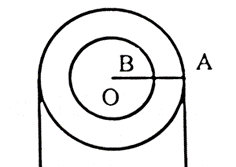
\includegraphics[scale=0.7]{../figs/VN10-2021-PH-TP006-1.png}
		\end{center}
		 Điểm A nằm ngoài vành của ròng rọc có vận tốc $v_\text A = \SI{2.4}{m/s}$. Điểm B cách A $\SI{10}{cm}$ có vận tốc $v_\text B = \SI{0.8}{m/s}$. Coi ròng rọc chuyển động tròn đều quanh trục. Tính tốc độ góc $\omega$ và bán kính $R$ của ròng rọc.
	}
	\loigiai
	{Hai điểm A và B có cùng tốc độ góc nên:
		$$\dfrac{R_\text{B}}{R_\text{A}} = \dfrac{v_\text{B}}{v_\text{A}}$$
		
		Với $R_\text{A} - R_\text{B} = \text{AB} = \SI{10}{cm}$, suy ra
		
		$$R_\text{A} =\SI{15}{cm}$$
		$$\omega=\SI{16}{rad/s}$$
	}
\end{enumerate}